\section{Simulation Analysis}
\label{sec:simulation}
The Ngspice Software was used to simulate the circuit.
We used Ngpice’s transient analysis mode to get v3(t)-v4(t), the dc output nodes, during 200 ms in order to observe 10 periods, take note that the frequency is 50Hz.
The initial time is 10 seconds in order to obtain the stationary part of the output, ignoring the trasient first part.
We had to set TMAX in transient analysis in ngspice, 
this tells the SPICE engine the max step it is allowed to take, but if it needs to take smaller steps it will.
The TMAX value was set to be 2e-4 in order to obtain at least 1000 points during the 200ms.
The table \ref{tab:simvalues} presents the values obtained.
The figures \ref{fig:acdc}, \ref{fig:envelope} and \ref{fig:deviation} present the dc ouput, the envelope
and the deviation value obtained in ngspice.

\vspace{10mm}

\subsection{Values obtained}

\vspace{10mm}

\begin{table}[ht]
  \centering
  \begin{tabular}{|c|c|}
    \hline    
    {\bf Quantities} & {\bf Volts / MU} \\ \hline
    \input{../sim/values_tab.tex}
  \end{tabular}
  \vspace{10mm}
  \caption{Average Voltage Value of DC Output (V). Ripple Value (Max-Min) (V). Cost of Circuit (MU). Merit of Circuit.}
  \label{tab:simvalues}
\end{table}


\newpage


\subsection{DC Output}

\begin{figure}[ht] \centering
\caption{DC Output for 200ms}
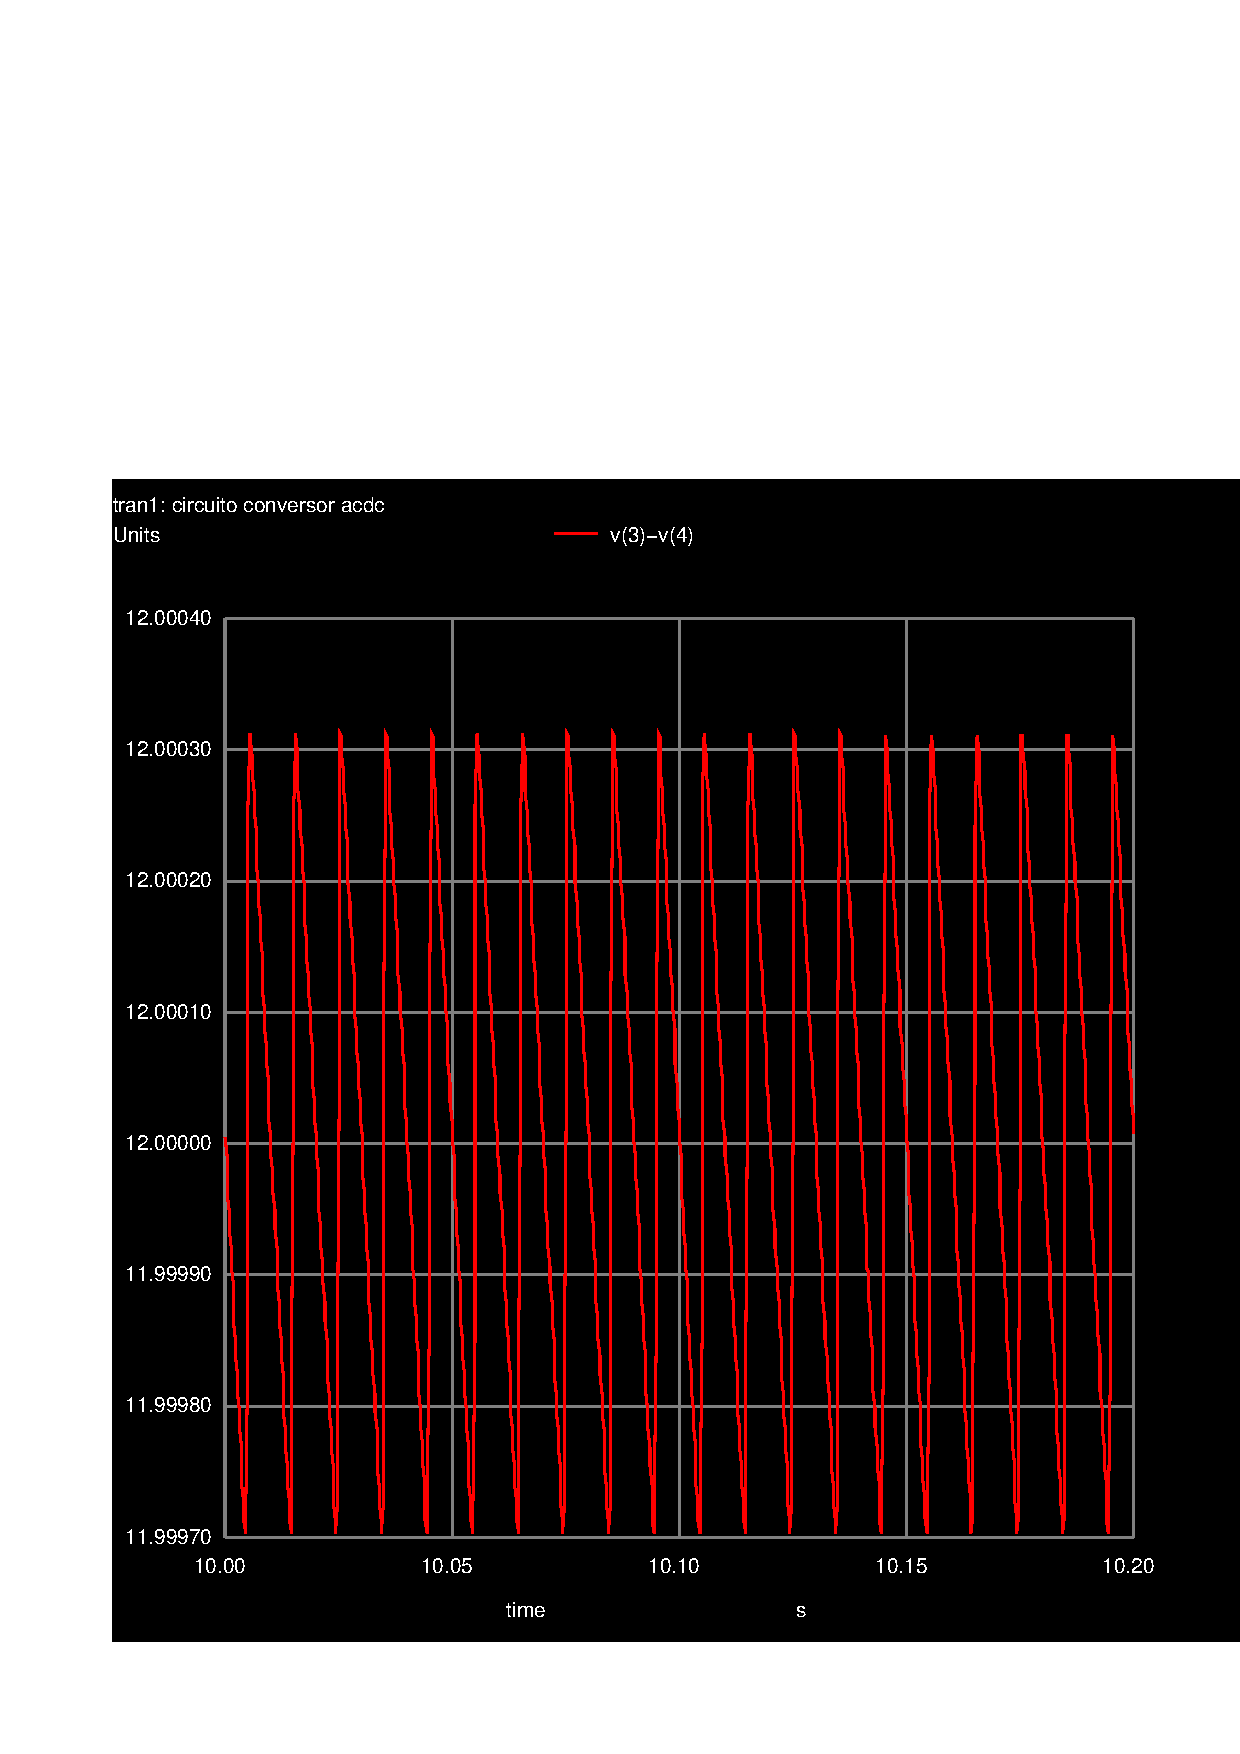
\includegraphics[width=0.8\linewidth]{../sim/acdc.pdf}
\label{fig:acdc}
\end{figure}

\newpage

\subsection{Output of the Envelope Detector}

\begin{figure}[ht] \centering
  \caption{Output of the Envelope Detector for 200ms}
  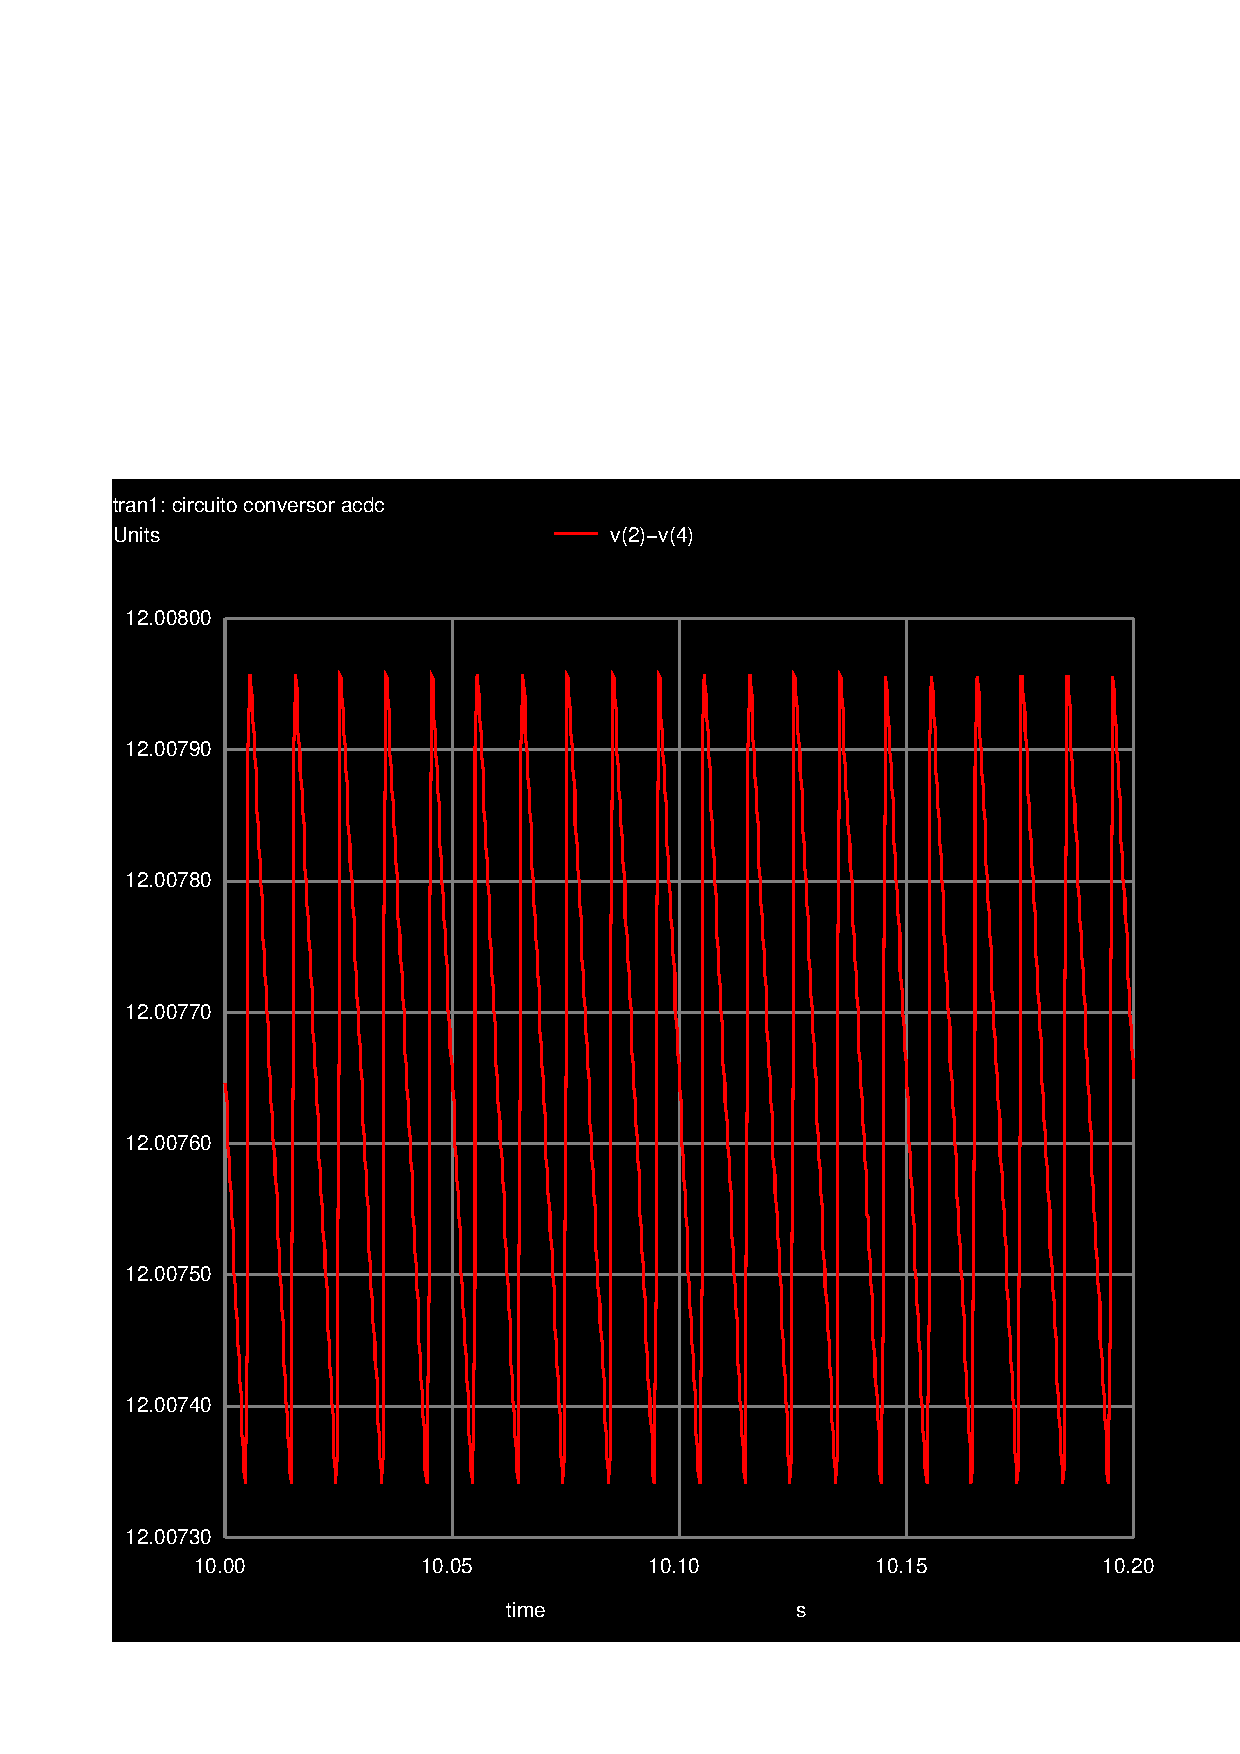
\includegraphics[width=0.8\linewidth]{../sim/envelope.pdf}
  \label{fig:envelope}
\end{figure}

\newpage

\subsection{Ouput Deviation}
\begin{figure}[ht] \centering
  \caption{Output AC component + DC deviation for 200ms in uVolts}
  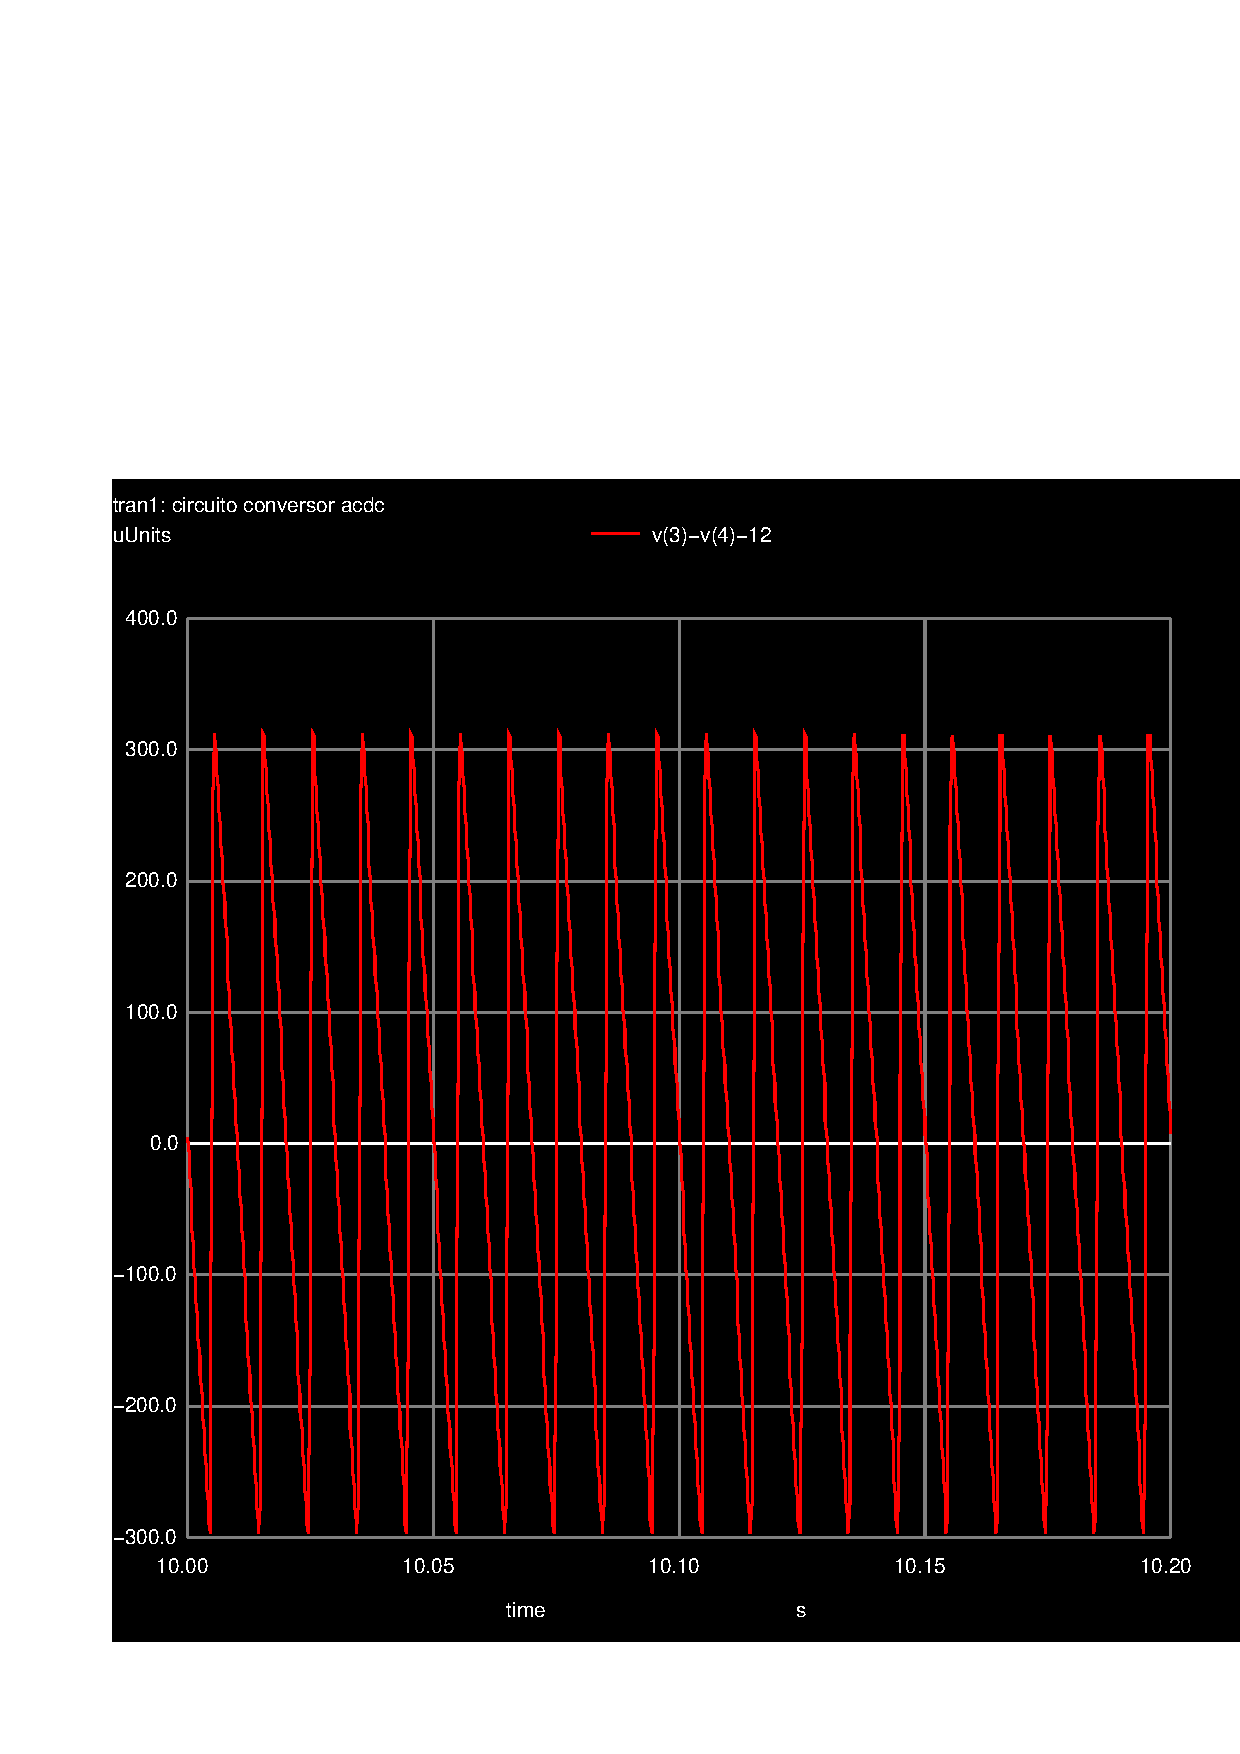
\includegraphics[width=0.8\linewidth]{../sim/deviation.pdf}
  \label{fig:deviation}
\end{figure}

\newpage







